\documentclass{standalone}
\usepackage{tikz}
\usetikzlibrary{patterns, positioning}


\begin{document}
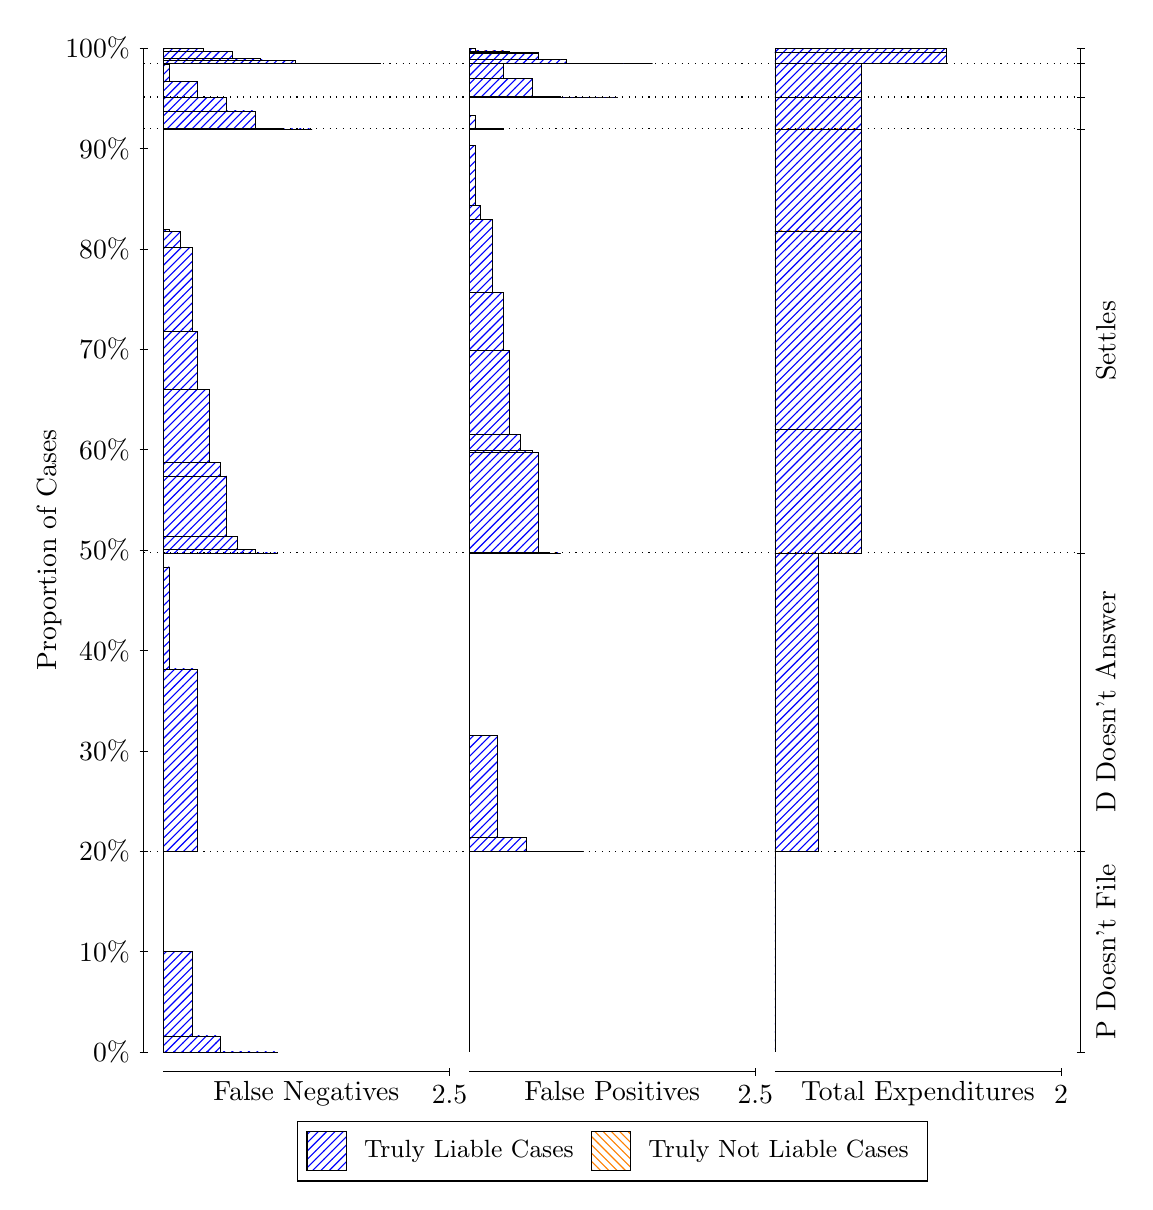
\begin{tikzpicture}
\draw[black, very thin] (1.5,1.75) -- (1.5,14.5);
\node[rotate=90, text=black, anchor=center] at (0.3, 8.125) {Proportion of Cases};
\draw[black, very thin] (1.45,1.75) -- (1.55,1.75);
\node[text=black, anchor=east] at (1.45, 1.75) {0\%};
\draw[black, very thin] (1.45,3.025) -- (1.55,3.025);
\node[text=black, anchor=east] at (1.45, 3.025) {10\%};
\draw[black, very thin] (1.45,4.3) -- (1.55,4.3);
\node[text=black, anchor=east] at (1.45, 4.3) {20\%};
\draw[black, very thin] (1.45,5.575) -- (1.55,5.575);
\node[text=black, anchor=east] at (1.45, 5.575) {30\%};
\draw[black, very thin] (1.45,6.85) -- (1.55,6.85);
\node[text=black, anchor=east] at (1.45, 6.85) {40\%};
\draw[black, very thin] (1.45,8.125) -- (1.55,8.125);
\node[text=black, anchor=east] at (1.45, 8.125) {50\%};
\draw[black, very thin] (1.45,9.4) -- (1.55,9.4);
\node[text=black, anchor=east] at (1.45, 9.4) {60\%};
\draw[black, very thin] (1.45,10.675) -- (1.55,10.675);
\node[text=black, anchor=east] at (1.45, 10.675) {70\%};
\draw[black, very thin] (1.45,11.95) -- (1.55,11.95);
\node[text=black, anchor=east] at (1.45, 11.95) {80\%};
\draw[black, very thin] (1.45,13.225) -- (1.55,13.225);
\node[text=black, anchor=east] at (1.45, 13.225) {90\%};
\draw[black, very thin] (1.45,14.5) -- (1.55,14.5);
\node[text=black, anchor=east] at (1.45, 14.5) {100\%};

\draw[black, very thin] (13.4,1.75) -- (13.4,14.5);
\draw[black, very thin] (13.35,1.75) -- (13.45,1.75);
\node[anchor=west] at (13.35, 1.75) {};
\draw[black, very thin] (13.35,4.2994) -- (13.45,4.2994);
\node[anchor=west] at (13.35, 4.2994) {};
\draw[black, very thin] (13.35,8.0891) -- (13.45,8.0891);
\node[anchor=west] at (13.35, 8.0891) {};
\draw[black, very thin] (13.35,13.474) -- (13.45,13.474);
\node[anchor=west] at (13.35, 13.474) {};
\draw[black, very thin] (13.35,13.878) -- (13.45,13.878);
\node[anchor=west] at (13.35, 13.878) {};
\draw[black, very thin] (13.35,14.304) -- (13.45,14.304);
\node[anchor=west] at (13.35, 14.304) {};
\draw[black, very thin] (13.35,14.5) -- (13.45,14.5);
\node[anchor=west] at (13.35, 14.5) {};

\draw[black, very thin, pattern color=blue, pattern=north east lines] (1.75,1.75) rectangle (3.2033,1.75);
\draw[black, very thin, pattern color=blue, pattern=north east lines] (1.75,1.75) rectangle (2.84,1.7517);
\draw[black, very thin, pattern color=blue, pattern=north east lines] (1.75,1.7517) rectangle (2.4767,1.954);
\draw[black, very thin, pattern color=blue, pattern=north east lines] (1.75,1.954) rectangle (2.1133,3.0265);
\draw[black, very thin, pattern color=orange, pattern=north west lines] (1.75,3.0265) rectangle (1.75,3.0265);
\draw[black, very thin, pattern color=blue, pattern=north east lines] (1.75,3.0265) rectangle (1.75,4.2994);
\draw[black, very thin, pattern color=blue, pattern=north east lines] (1.75,4.2994) rectangle (2.186,6.6138);
\draw[black, very thin, pattern color=blue, pattern=north east lines] (1.75,6.6138) rectangle (1.8227,7.911);
\draw[black, very thin, pattern color=orange, pattern=north west lines] (1.75,7.911) rectangle (1.75,7.911);
\draw[black, very thin, pattern color=blue, pattern=north east lines] (1.75,7.911) rectangle (1.75,8.0891);
\draw[black, very thin, pattern color=blue, pattern=north east lines] (1.75,8.0891) rectangle (3.2033,8.0891);
\draw[black, very thin, pattern color=blue, pattern=north east lines] (1.75,8.0891) rectangle (3.058,8.0894);
\draw[black, very thin, pattern color=blue, pattern=north east lines] (1.75,8.0894) rectangle (2.9127,8.1284);
\draw[black, very thin, pattern color=blue, pattern=north east lines] (1.75,8.1284) rectangle (2.84,8.1289);
\draw[black, very thin, pattern color=blue, pattern=north east lines] (1.75,8.1289) rectangle (2.6947,8.2967);
\draw[black, very thin, pattern color=blue, pattern=north east lines] (1.75,8.2967) rectangle (2.5493,9.0656);
\draw[black, very thin, pattern color=blue, pattern=north east lines] (1.75,9.0656) rectangle (2.4767,9.2405);
\draw[black, very thin, pattern color=blue, pattern=north east lines] (1.75,9.2405) rectangle (2.3313,10.163);
\draw[black, very thin, pattern color=blue, pattern=north east lines] (1.75,10.163) rectangle (2.186,10.898);
\draw[black, very thin, pattern color=blue, pattern=north east lines] (1.75,10.898) rectangle (2.1133,11.969);
\draw[black, very thin, pattern color=blue, pattern=north east lines] (1.75,11.969) rectangle (1.968,12.173);
\draw[black, very thin, pattern color=blue, pattern=north east lines] (1.75,12.173) rectangle (1.8227,12.199);
\draw[black, very thin, pattern color=orange, pattern=north west lines] (1.75,12.199) rectangle (1.75,12.199);
\draw[black, very thin, pattern color=blue, pattern=north east lines] (1.75,12.199) rectangle (1.75,13.474);
\draw[black, very thin, pattern color=blue, pattern=north east lines] (1.75,13.474) rectangle (3.6393,13.474);
\draw[black, very thin, pattern color=blue, pattern=north east lines] (1.75,13.474) rectangle (3.276,13.479);
\draw[black, very thin, pattern color=blue, pattern=north east lines] (1.75,13.479) rectangle (2.9127,13.703);
\draw[black, very thin, pattern color=blue, pattern=north east lines] (1.75,13.703) rectangle (2.5493,13.876);
\draw[black, very thin, pattern color=blue, pattern=north east lines] (1.75,13.876) rectangle (2.186,13.878);
\draw[black, very thin, pattern color=orange, pattern=north west lines] (1.75,13.878) rectangle (1.75,13.878);
\draw[black, very thin, pattern color=blue, pattern=north east lines] (1.75,13.878) rectangle (2.186,14.072);
\draw[black, very thin, pattern color=blue, pattern=north east lines] (1.75,14.072) rectangle (1.8227,14.295);
\draw[black, very thin, pattern color=orange, pattern=north west lines] (1.75,14.295) rectangle (1.75,14.295);
\draw[black, very thin, pattern color=blue, pattern=north east lines] (1.75,14.295) rectangle (1.75,14.304);
\draw[black, very thin, pattern color=blue, pattern=north east lines] (1.75,14.304) rectangle (4.5113,14.304);
\draw[black, very thin, pattern color=blue, pattern=north east lines] (1.75,14.304) rectangle (4.148,14.304);
\draw[black, very thin, pattern color=blue, pattern=north east lines] (1.75,14.304) rectangle (3.7847,14.309);
\draw[black, very thin, pattern color=blue, pattern=north east lines] (1.75,14.309) rectangle (3.712,14.309);
\draw[black, very thin, pattern color=blue, pattern=north east lines] (1.75,14.309) rectangle (3.4213,14.339);
\draw[black, very thin, pattern color=blue, pattern=north east lines] (1.75,14.339) rectangle (3.3487,14.339);
\draw[black, very thin, pattern color=blue, pattern=north east lines] (1.75,14.339) rectangle (3.058,14.35);
\draw[black, very thin, pattern color=blue, pattern=north east lines] (1.75,14.35) rectangle (2.9853,14.365);
\draw[black, very thin, pattern color=blue, pattern=north east lines] (1.75,14.365) rectangle (2.6947,14.365);
\draw[black, very thin, pattern color=blue, pattern=north east lines] (1.75,14.365) rectangle (2.622,14.453);
\draw[black, very thin, pattern color=blue, pattern=north east lines] (1.75,14.453) rectangle (2.3313,14.453);
\draw[black, very thin, pattern color=blue, pattern=north east lines] (1.75,14.453) rectangle (2.2587,14.498);
\draw[black, very thin, pattern color=blue, pattern=north east lines] (1.75,14.498) rectangle (1.8953,14.5);
\draw[black, very thin, pattern color=orange, pattern=north west lines] (1.75,14.5) rectangle (1.75,14.5);
\draw[black, very thin, pattern color=blue, pattern=north east lines] (1.75,14.5) rectangle (1.75,14.5);
\draw[black, very thin, pattern color=orange, pattern=north west lines] (5.6333,1.75) rectangle (5.6333,1.75);
\draw[black, very thin, pattern color=blue, pattern=north east lines] (5.6333,1.75) rectangle (5.6333,4.2994);
\draw[black, very thin, pattern color=orange, pattern=north west lines] (5.6333,4.2994) rectangle (7.0867,4.2994);
\draw[black, very thin, pattern color=blue, pattern=north east lines] (5.6333,4.2994) rectangle (7.0867,4.2994);
\draw[black, very thin, pattern color=blue, pattern=north east lines] (5.6333,4.2994) rectangle (6.7233,4.2998);
\draw[black, very thin, pattern color=blue, pattern=north east lines] (5.6333,4.2998) rectangle (6.36,4.4775);
\draw[black, very thin, pattern color=blue, pattern=north east lines] (5.6333,4.4775) rectangle (5.9967,5.7747);
\draw[black, very thin, pattern color=blue, pattern=north east lines] (5.6333,5.7747) rectangle (5.6333,8.0891);
\draw[black, very thin, pattern color=orange, pattern=north west lines] (5.6333,8.0891) rectangle (6.796,8.0891);
\draw[black, very thin, pattern color=blue, pattern=north east lines] (5.6333,8.0891) rectangle (6.796,8.0891);
\draw[black, very thin, pattern color=orange, pattern=north west lines] (5.6333,8.0891) rectangle (6.6507,8.0891);
\draw[black, very thin, pattern color=blue, pattern=north east lines] (5.6333,8.0891) rectangle (6.6507,8.0911);
\draw[black, very thin, pattern color=orange, pattern=north west lines] (5.6333,8.0911) rectangle (6.5053,8.0911);
\draw[black, very thin, pattern color=blue, pattern=north east lines] (5.6333,8.0911) rectangle (6.5053,9.3641);
\draw[black, very thin, pattern color=blue, pattern=north east lines] (5.6333,9.3641) rectangle (6.4327,9.3899);
\draw[black, very thin, pattern color=blue, pattern=north east lines] (5.6333,9.3899) rectangle (6.2873,9.5936);
\draw[black, very thin, pattern color=blue, pattern=north east lines] (5.6333,9.5936) rectangle (6.142,10.665);
\draw[black, very thin, pattern color=blue, pattern=north east lines] (5.6333,10.665) rectangle (6.0693,11.4);
\draw[black, very thin, pattern color=blue, pattern=north east lines] (5.6333,11.4) rectangle (5.924,12.322);
\draw[black, very thin, pattern color=blue, pattern=north east lines] (5.6333,12.322) rectangle (5.7787,12.497);
\draw[black, very thin, pattern color=blue, pattern=north east lines] (5.6333,12.497) rectangle (5.706,13.266);
\draw[black, very thin, pattern color=blue, pattern=north east lines] (5.6333,13.266) rectangle (5.6333,13.474);
\draw[black, very thin, pattern color=orange, pattern=north west lines] (5.6333,13.474) rectangle (6.0693,13.474);
\draw[black, very thin, pattern color=blue, pattern=north east lines] (5.6333,13.474) rectangle (6.0693,13.476);
\draw[black, very thin, pattern color=blue, pattern=north east lines] (5.6333,13.476) rectangle (5.706,13.649);
\draw[black, very thin, pattern color=blue, pattern=north east lines] (5.6333,13.649) rectangle (5.6333,13.878);
\draw[black, very thin, pattern color=orange, pattern=north west lines] (5.6333,13.878) rectangle (7.5227,13.878);
\draw[black, very thin, pattern color=blue, pattern=north east lines] (5.6333,13.878) rectangle (7.5227,13.878);
\draw[black, very thin, pattern color=blue, pattern=north east lines] (5.6333,13.878) rectangle (7.1593,13.878);
\draw[black, very thin, pattern color=blue, pattern=north east lines] (5.6333,13.878) rectangle (6.796,13.887);
\draw[black, very thin, pattern color=blue, pattern=north east lines] (5.6333,13.887) rectangle (6.4327,14.11);
\draw[black, very thin, pattern color=blue, pattern=north east lines] (5.6333,14.11) rectangle (6.0693,14.304);
\draw[black, very thin, pattern color=orange, pattern=north west lines] (5.6333,14.304) rectangle (7.9587,14.304);
\draw[black, very thin, pattern color=blue, pattern=north east lines] (5.6333,14.304) rectangle (7.9587,14.304);
\draw[black, very thin, pattern color=orange, pattern=north west lines] (5.6333,14.304) rectangle (7.5953,14.304);
\draw[black, very thin, pattern color=blue, pattern=north east lines] (5.6333,14.304) rectangle (7.5953,14.304);
\draw[black, very thin, pattern color=orange, pattern=north west lines] (5.6333,14.304) rectangle (7.232,14.304);
\draw[black, very thin, pattern color=blue, pattern=north east lines] (5.6333,14.304) rectangle (7.232,14.307);
\draw[black, very thin, pattern color=blue, pattern=north east lines] (5.6333,14.307) rectangle (6.8687,14.352);
\draw[black, very thin, pattern color=orange, pattern=north west lines] (5.6333,14.352) rectangle (6.8687,14.352);
\draw[black, very thin, pattern color=blue, pattern=north east lines] (5.6333,14.352) rectangle (6.8687,14.352);
\draw[black, very thin, pattern color=orange, pattern=north west lines] (5.6333,14.352) rectangle (6.796,14.352);
\draw[black, very thin, pattern color=blue, pattern=north east lines] (5.6333,14.352) rectangle (6.796,14.352);
\draw[black, very thin, pattern color=blue, pattern=north east lines] (5.6333,14.352) rectangle (6.5053,14.439);
\draw[black, very thin, pattern color=blue, pattern=north east lines] (5.6333,14.439) rectangle (6.5053,14.44);
\draw[black, very thin, pattern color=orange, pattern=north west lines] (5.6333,14.44) rectangle (6.4327,14.44);
\draw[black, very thin, pattern color=blue, pattern=north east lines] (5.6333,14.44) rectangle (6.4327,14.44);
\draw[black, very thin, pattern color=blue, pattern=north east lines] (5.6333,14.44) rectangle (6.142,14.447);
\draw[black, very thin, pattern color=blue, pattern=north east lines] (5.6333,14.447) rectangle (6.142,14.455);
\draw[black, very thin, pattern color=blue, pattern=north east lines] (5.6333,14.455) rectangle (6.0693,14.465);
\draw[black, very thin, pattern color=orange, pattern=north west lines] (5.6333,14.465) rectangle (6.0693,14.465);
\draw[black, very thin, pattern color=blue, pattern=north east lines] (5.6333,14.465) rectangle (6.0693,14.465);
\draw[black, very thin, pattern color=blue, pattern=north east lines] (5.6333,14.465) rectangle (5.7787,14.465);
\draw[black, very thin, pattern color=blue, pattern=north east lines] (5.6333,14.465) rectangle (5.7787,14.465);
\draw[black, very thin, pattern color=blue, pattern=north east lines] (5.6333,14.465) rectangle (5.706,14.495);
\draw[black, very thin, pattern color=blue, pattern=north east lines] (5.6333,14.495) rectangle (5.706,14.496);
\draw[black, very thin, pattern color=blue, pattern=north east lines] (5.6333,14.496) rectangle (5.6333,14.5);
\draw[black, very thin, pattern color=orange, pattern=north west lines] (9.5167,1.75) rectangle (9.5167,1.75);
\draw[black, very thin, pattern color=blue, pattern=north east lines] (9.5167,1.75) rectangle (9.5167,4.2994);
\draw[black, very thin, pattern color=orange, pattern=north west lines] (9.5167,4.2994) rectangle (10.062,4.2994);
\draw[black, very thin, pattern color=blue, pattern=north east lines] (9.5167,4.2994) rectangle (10.062,8.0891);
\draw[black, very thin, pattern color=orange, pattern=north west lines] (9.5167,8.0891) rectangle (10.607,8.0891);
\draw[black, very thin, pattern color=blue, pattern=north east lines] (9.5167,8.0891) rectangle (10.607,9.6575);
\draw[black, very thin, pattern color=orange, pattern=north west lines] (9.5167,9.6575) rectangle (10.607,9.6575);
\draw[black, very thin, pattern color=blue, pattern=north east lines] (9.5167,9.6575) rectangle (10.607,12.177);
\draw[black, very thin, pattern color=orange, pattern=north west lines] (9.5167,12.177) rectangle (10.607,12.177);
\draw[black, very thin, pattern color=blue, pattern=north east lines] (9.5167,12.177) rectangle (10.607,13.474);
\draw[black, very thin, pattern color=orange, pattern=north west lines] (9.5167,13.474) rectangle (10.607,13.474);
\draw[black, very thin, pattern color=blue, pattern=north east lines] (9.5167,13.474) rectangle (10.607,13.878);
\draw[black, very thin, pattern color=orange, pattern=north west lines] (9.5167,13.878) rectangle (10.607,13.878);
\draw[black, very thin, pattern color=blue, pattern=north east lines] (9.5167,13.878) rectangle (10.607,14.304);
\draw[black, very thin, pattern color=orange, pattern=north west lines] (9.5167,14.304) rectangle (11.697,14.304);
\draw[black, very thin, pattern color=blue, pattern=north east lines] (9.5167,14.304) rectangle (11.697,14.446);
\draw[black, very thin, pattern color=orange, pattern=north west lines] (9.5167,14.446) rectangle (11.697,14.446);
\draw[black, very thin, pattern color=blue, pattern=north east lines] (9.5167,14.446) rectangle (11.697,14.5);
\draw[black, dotted] (1.5,4.2994) -- (13.4,4.2994);
\draw[black, dotted] (1.5,8.0891) -- (13.4,8.0891);
\draw[black, dotted] (1.5,13.474) -- (13.4,13.474);
\draw[black, dotted] (1.5,13.878) -- (13.4,13.878);
\draw[black, dotted] (1.5,14.304) -- (13.4,14.304);
\draw[black, very thin] (1.75,1.5) -- (5.3833,1.5);
\node[text=black, anchor=north] at (3.5667, 1.5) {False Negatives};
\draw[black, very thin] (5.3833,1.45) -- (5.3833,1.55);
\node[text=black, anchor=north] at (5.3833, 1.45) {2.5};

\draw[black, very thin] (5.6333,1.5) -- (9.2667,1.5);
\node[text=black, anchor=north] at (7.45, 1.5) {False Positives};
\draw[black, very thin] (9.2667,1.45) -- (9.2667,1.55);
\node[text=black, anchor=north] at (9.2667, 1.45) {2.5};

\draw[black, very thin] (9.5167,1.5) -- (13.15,1.5);
\node[text=black, anchor=north] at (11.333, 1.5) {Total Expenditures};
\draw[black, very thin] (13.15,1.45) -- (13.15,1.55);
\node[text=black, anchor=north] at (13.15, 1.45) {2};

\node[text=black, centered, rotate=90] at (13.72, 3.0247) {P Doesn't File};
\node[text=black, centered, rotate=90] at (13.72, 6.1942) {D Doesn't Answer};
\node[text=black, centered, rotate=90] at (13.72, 10.781) {Settles};




\draw (7.449999999999999,1.5) node[draw=none] (baseCoordinate) {};
\begin{scope}[align=center]
        \matrix[scale=0.5, draw=black, below=0.5cm of baseCoordinate, nodes={draw}, column sep=0.1cm]{
            \node[rectangle, draw, minimum width=0.5cm, minimum height=0.5cm, pattern color=blue, pattern=north east lines] {}; &
            \node[draw=none, font=\small, text=black] (B) {Truly Liable Cases}; &
            \node[rectangle, draw, minimum width=0.5cm, minimum height=0.5cm, pattern color=orange, pattern=north west lines] {}; &
            \node[draw=none, font=\small, text=black] (B) {Truly Not Liable Cases}; \\
            };
\end{scope}

\end{tikzpicture}
\end{document}